% \documentclass{beamer}
% \usetheme{metropolis}           % Use metropolis theme
% \title{Visual assessments of Postural
% Orientation Errors using
% ensembles of Deep Neural
% Networks}
% \date{\today}
% \author{Filip Kronström}
% \institute{Lund University}
% \begin{document}
%   \maketitle
%   \section{First Section}
%   \begin{frame}{First Frame}
%     Hello, world!
%   \end{frame}
% \end{document}

\documentclass[10pt]{beamer}

\usetheme{metropolis}
\usepackage{appendixnumberbeamer}
% \usepackage{setspace}

\usepackage{booktabs}
\usepackage[scale=2]{ccicons}
% \usepackage{footmisc}
\usepackage{scrextend}
% \usepackage{setspace}
\usepackage{pgfplots}
% \usepackage{multimedia}
\usepackage{animate}
\usepgfplotslibrary{dateplot}
% \addbibresource{files/bibtex/pres_bib.bib}

% \setsansfont{Ubuntu}
% \setmonofont{Ubuntu Mono}

\usepackage{xspace}
% \usepackage{subcaption}
\newcommand{\themename}{\textbf{\textsc{metropolis}}\xspace}
% \renewcommand{\small}{\footnotesize}
\renewcommand{\footnotesize}{\tiny}
\title{Visual assessments of\\Postural
Orientation\\Errors using
ensembles\\of Deep Neural
Networks}
\subtitle{Master's Thesis}
\date{\today}
\author[me]{\textbf{\large Filip Kronström}\\[1.5mm]Supervisors: A. Jakobsson\footnote{Centre for Mathematical Sciences, Mathematical Statistics, Lund University}, J. Älmqvist\footnote{\label{hs}Department of Health Sciences, Lund University}, E. Ageberg$^{\ref{hs}}$, M. Creaby\footnote{School of Exercise Science, Australian Catholic University \newline}}
\institute{\large Faculty of Engineering, Lund University}
\titlegraphic{\hfill
\includegraphics[height=2.6cm]{files/figs/presentation/lth_logo_en.eps}}

\begin{document}

\maketitle
% \footnotetext[4]{\newline}

\begin{frame}{Agenda}
  \setbeamertemplate{section in toc}[sections numbered]
  \tableofcontents[hideallsubsections]
\end{frame}

\section{Introduction}
\begin{frame}[fragile]{Sports injuries}
  % lol\footnote{LaBella et al., Anterior Cruciate Ligament Injuries: Diagnosis, Treatment, and Prevention. 2014}
    \begin{columns}[T,onlytextwidth]
      \column{0.45\textwidth}
        {\small50\% of amateur football players in Denmark experience hip/groin pain during season\footnotemark.}
      \column{0.45\textwidth}
        {\small Around 8000 yearly Anterior cruciate ligament injuries in Sweden\footnotemark.}
    \end{columns}
    \begin{figure}
      \centering
      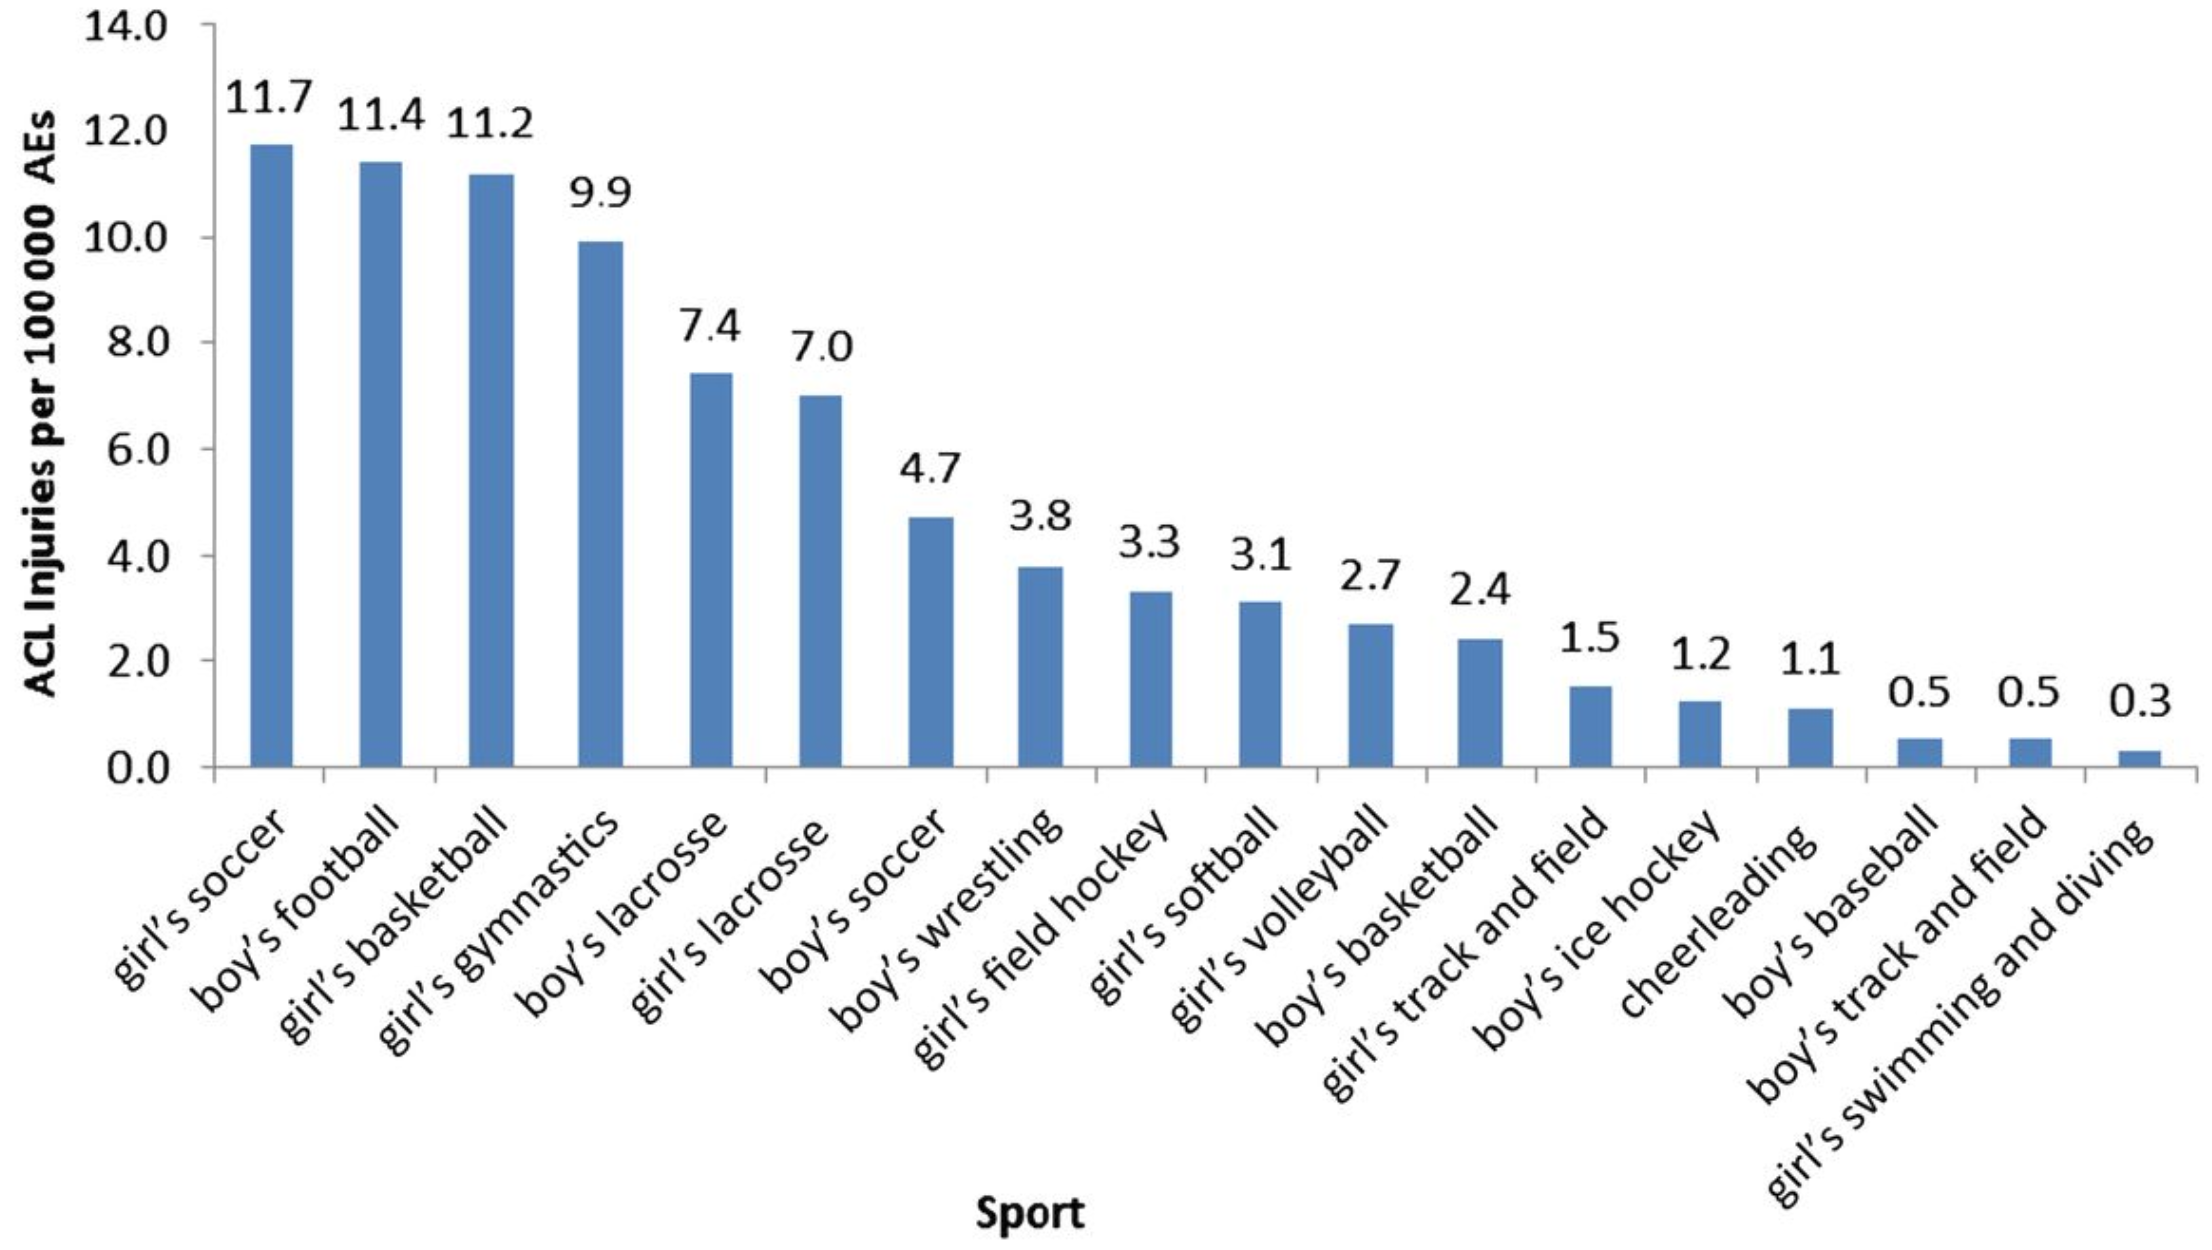
\includegraphics[width=0.75\textwidth]{files/figs/presentation/acl-injury-per-ae.png}
      % \caption[Caption for LOF]{Injury rates among high school students, per 100 000 athlete exposures\footnote{LaBella et al., Anterior Cruciate Ligament Injuries: Diagnosis, Treatment, and Prevention. 2014}.}

      {\scriptsize\textbf{Figure 1:} Injury rates among high school students, per 100 000 athlete exposures\footnotemark.}
      % \label{}
    \end{figure}


\footnotetext[1]{Thorborg et al., Prevalence
and severity of hip and groin pain in sub-elite male football: a cross-sectional cohort study of 695 players. 2017}
\footnotetext[2]{Svenska korsbandsregistret, Årsrapport 2019. 2020}
\footnotetext[3]{LaBella et al., Anterior Cruciate Ligament Injuries: Diagnosis, Treatment, and Prevention. 2014}

\end{frame}

\begin{frame}[c,fragile]{Anterior cruciate ligament injury and rehabilitation}
  \begin{columns}[c,onlytextwidth]
    \column{0.45\textwidth}
      \begin{itemize}
        % \small
          \item Regular injury mechanism is sudden changes in direction or velocity while knee is bearing weight\footnotemark.
          \item Rehabilitation typically up to 2 years\footnotemark.
          \item Increased long and short term risk of, e.g., osteoarthritis\footnotemark, joint instability\footnotemark, and re-injury\footnotemark.
      \end{itemize}

    \column{0.55\textwidth}
    \begin{figure}
      \centering
      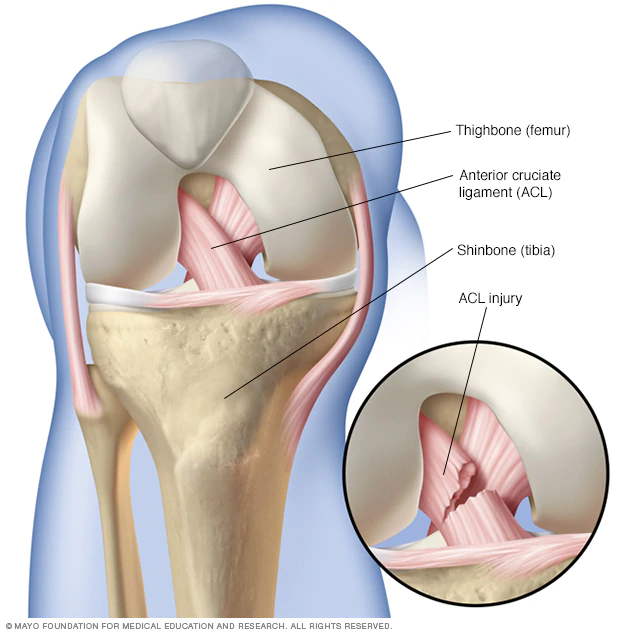
\includegraphics[width=0.9\textwidth]{files/figs/intro/acl.png}
      % \caption{}
      % \label{}

      {\scriptsize\textbf{Figure 2:} Illustration of ACL in the knee\footnotemark.}
    \end{figure}

  \end{columns}

  \footnotetext[4]{Wetters et al., Mechanism of Injury and Risk Factors for Anterior Cruciate Ligament Injury. 2016}
  \footnotetext[5]{Nagelli and Hewett, Should Return to Sport be Delayed Until 2 Years After Anterior Cruciate Ligament Reconstruction? Biological and Functional Considerations. 2017}
  \footnotetext[6]{Mayo Clinic, \url{https://www.mayoclinic.org/diseases-conditions/acl-injury/symptoms-causes/syc-20350738}}
  \footnotetext[7]{Wetters et al., Mechanism of Injury and Risk Factors for Anterior Cruciate Ligament Injury. 2016}
  \footnotetext[8]{Nagelli and Hewett, Should Return to Sport be Delayed Until 2 Years After Anterior Cruciate Ligament Reconstruction? Biological and Functional Considerations. 2017}
  \footnotetext[9]{Mayo Clinic, \url{https://www.mayoclinic.org/diseases-conditions/acl-injury/symptoms-causes/syc-20350738}}

\end{frame}

\begin{frame}[fragile]{Postural Orientation Errors}
  \begin{columns}[T,onlytextwidth]
    \centering
    \column{0.55\textwidth}
  \begin{columns}[T,onlytextwidth]
      \column{0.49\textwidth}

      \begin{figure}
        \raggedleft
        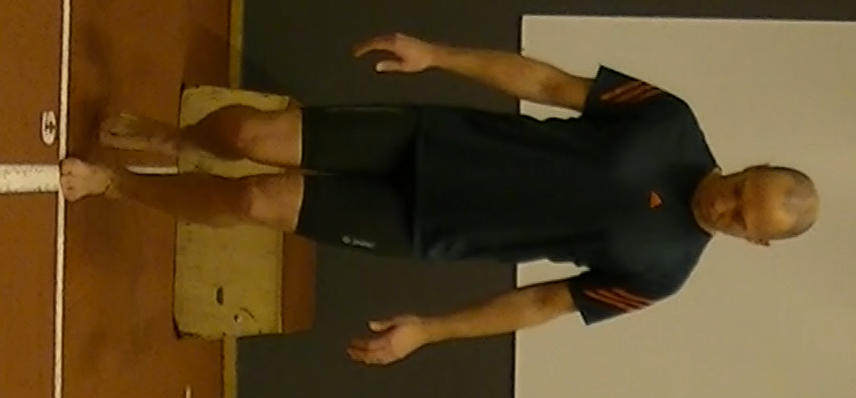
\includegraphics[angle=90,height=0.7\textheight]{files/figs/presentation/good-poe.png}
        % \caption{}
        % \label{}
      \end{figure}

      \column{0.49\textwidth}
      \begin{figure}
        \raggedright
        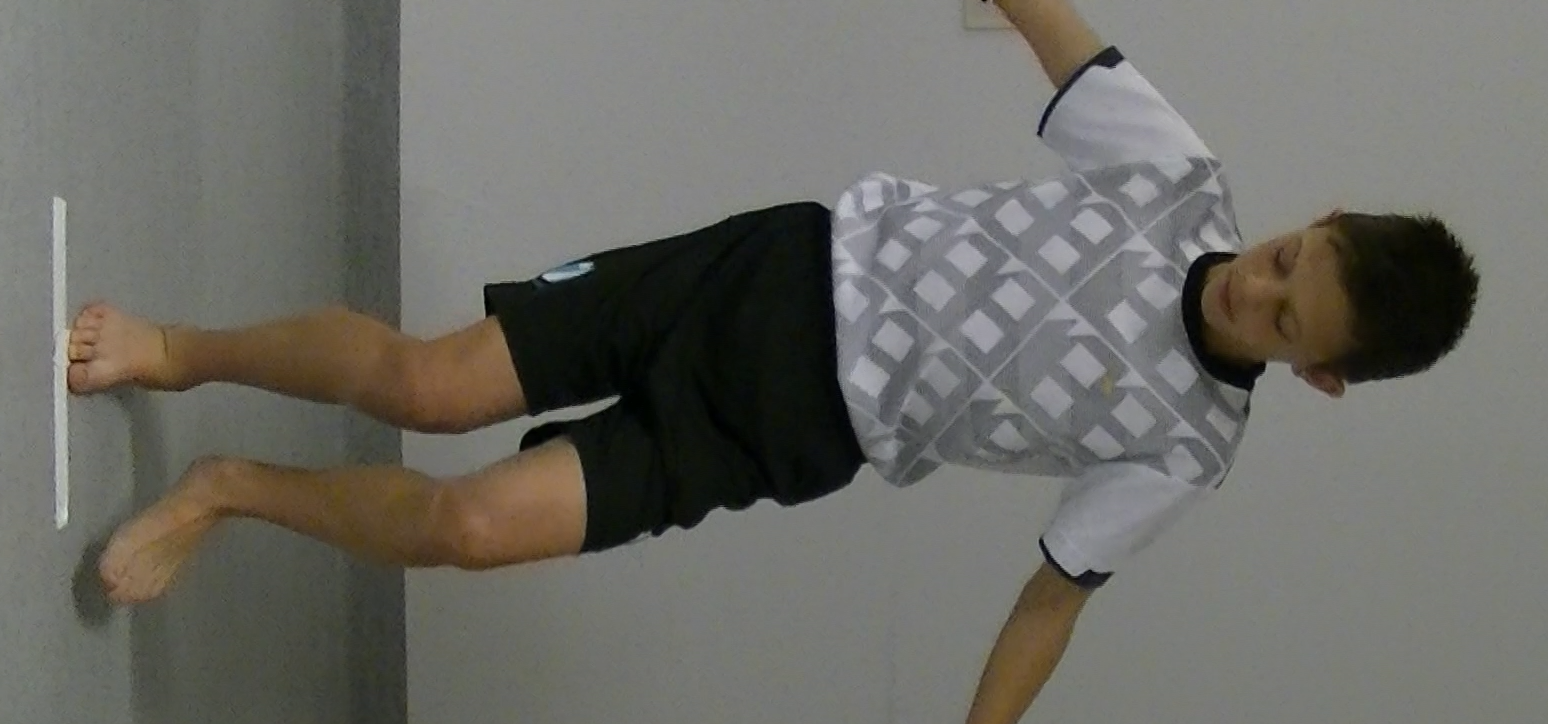
\includegraphics[angle=90,height=0.7\textheight]{files/figs/presentation/poor-poe.png}
        % \caption{}
        % \label{}
      \end{figure}
  \end{columns}
  \vspace{0.1cm}
  {\scriptsize\textbf{Figure 3:} Examples of maintained (left) and altered postural orientation (right) during a single leg squat. \newline}
  \column{0.45\textwidth}
  \begin{itemize}
    \item Ability to uphold alignment of body parts.
    \item Altered PO - seen to increase risk of re-injury.
    \item No established and feasible method to assess for clinical use.
    \item Proposed methods where experts assess motions on videos - time consuming\footnotemark.
  \end{itemize}
  \end{columns}

  \footnotetext[10]{\hspace Nae et al., Extended Version of a Test Battery for Visual Assessment of Postural Orientation Errors: Face Validity, Internal Consistency, and Reliability. 2020}

  % \begin{figure}
  %   \centering
  %   \begin{subfigure}[t]{0.45/textwidth}
  %       \raggedleft
  %       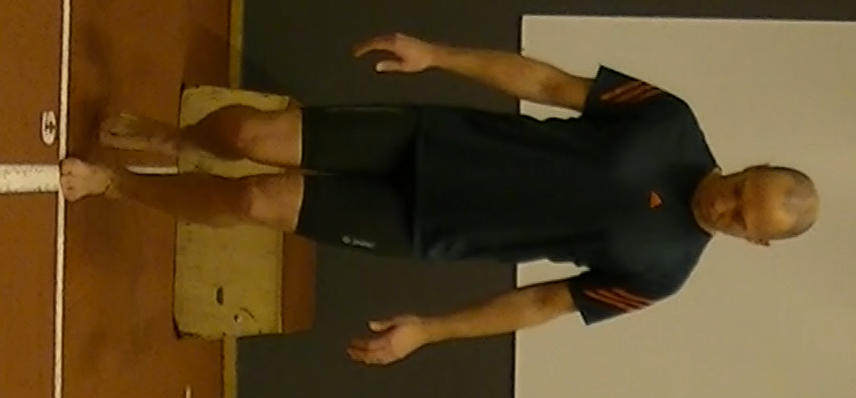
\includegraphics[height=0.5\textheight,angle=90]{files/figs/presentation/good-poe.png}
  %   \end{subfigure}
  %   ~
  %   \begin{subfigure}[t]{0.45\textwidth}
  %     \raggedright
  %     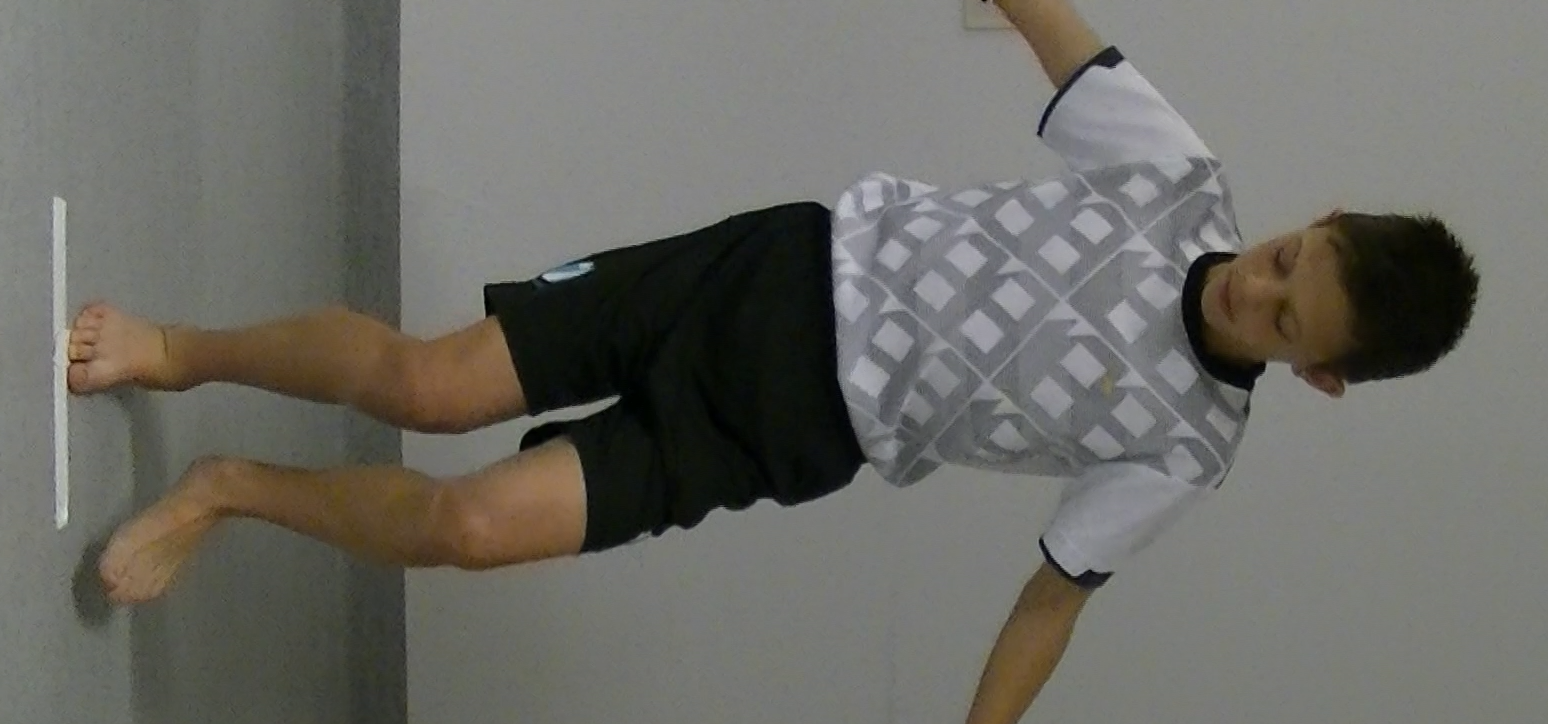
\includegraphics[height=0.5\textheight,angle=90]{files/figs/presentation/poor-poe.png}
  %   \end{subfigure}
    % 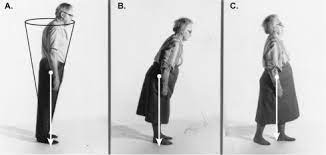
\includegraphics[height=0.5\textheight]{files/figs/presentation/postural-orientation.jpeg}
    %
    % {\scriptsize\textbf{Figure 3:} Examples of postural orientation\footnotemark}
    % \caption{}
    % \label{}
  % \end{figure}

% \footnotetext[10]{Horak, Postural orientation and equilibrium: what do we need to know about neural control of balance to prevent falls?. 2006}
\end{frame}

\begin{frame}[fragile]{ngt om avgransningar och de olika poesen}
  wtf?
\end{frame}

\section{Methods}

\begin{frame}[fragile]{System overview}
    \begin{figure}
      \centering
      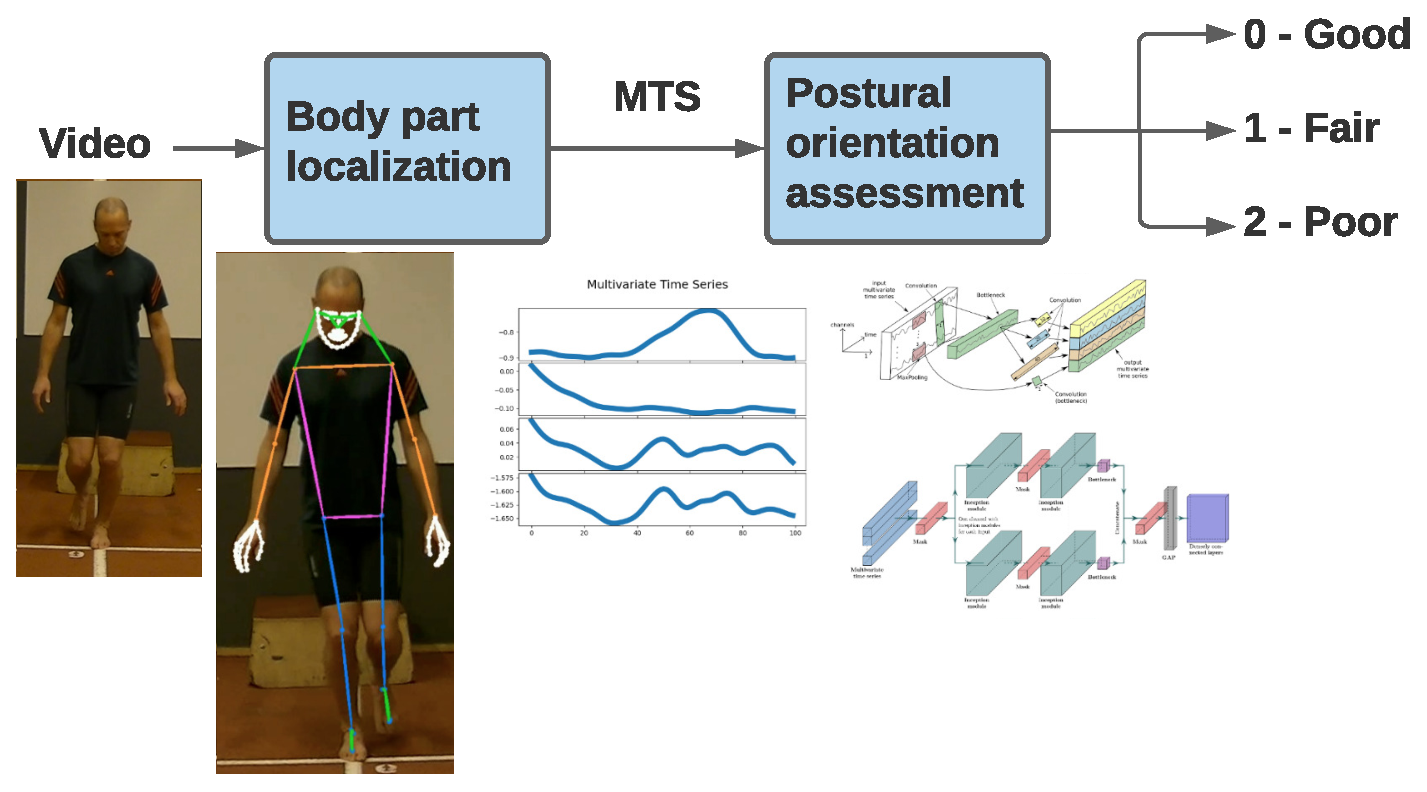
\includegraphics[width=\textwidth]{files/figs/presentation/sys-overview.eps}

      {\scriptsize\textbf{Figure 4}}
      % \caption{}
      % \label{}
    \end{figure}
\end{frame}

\begin{frame}[fragile]{Body part localization}
  \begin{columns}[T,onlytextwidth]
      \column{0.45\textwidth}
      % \animategraphics[loop,controls={play,stop},height=0.7\textheight]{25}{files/figs/presentation/sls06-pngs/sls06L-imgs-}{0}{539}

      % embedda video pa ngt satt

      \column{0.55\textwidth}
      \begin{itemize}
        \item Built upon MMPose framework\footnotemark.
        \item HRNet\footnotemark with DARK-pose\footnotemark trained on COCO-wholebody dataset used for pose estimation.
        \item Outputs 133 keypoint coordinates.
      \end{itemize}
  \end{columns}

  \footnotetext[11]{MMPose - OpenMMLab, \url{https://github.com/open-mmlab/mmpose}}
  \footnotetext[12]{Sun et al., Deep high-resolution representation learning for human pose estimation. 2019}
  \footnotetext[13]{Zhang et al., Distribution-Aware Coordinate Representation for Human Pose Estimation. 2020}


  % \movie[height=\textheight,poster]{}{files/figs/presentation/06-SLS-L-25.mp4}
\end{frame}
% prata om hur pixel space reduceras till keypoint space,
%

\begin{frame}[fragile]{Time series classification - Network architectures}
  \begin{columns}[c,onlytextwidth]
    \column{0.55\textwidth}
    \begin{figure}
      \centering
      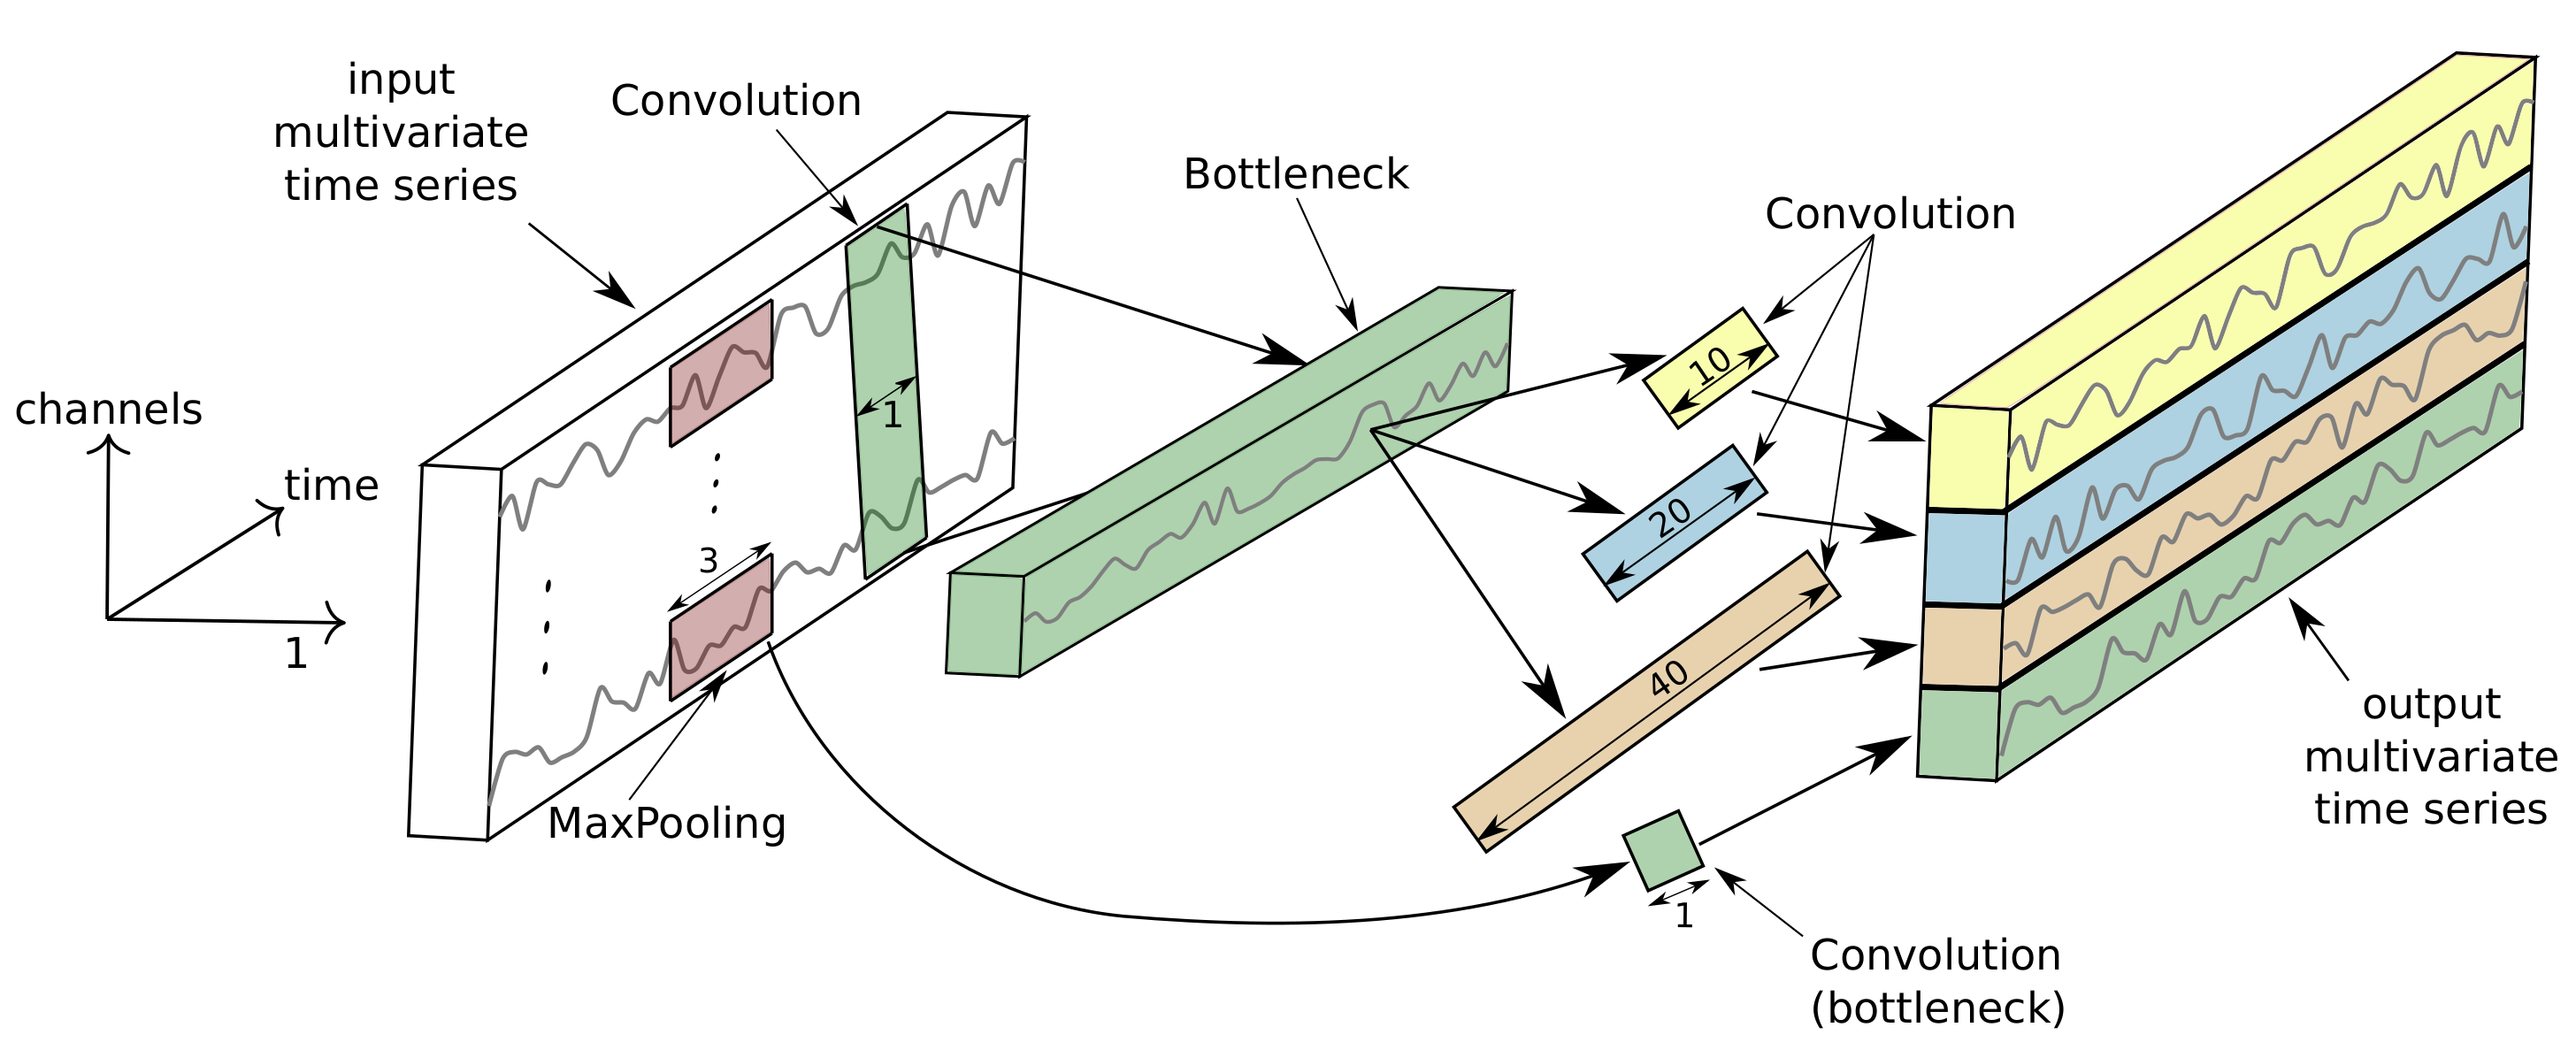
\includegraphics[width=\textwidth]{files/figs/tsc/inception-time-module.png}
      {\scriptsize\textbf{Figure 5:} InceptionTime module.}
      % \caption{}
      % \label{}
    \end{figure}

  \column{0.4\textwidth}
  \begin{block}{IncetionTime\footnotemark}
    Modules with convolutions of different lengths, global average pooling, and densely connected layers for classification.
  \end{block}
  \end{columns}

  \begin{columns}[c,onlytextwidth]
    \column{0.55\textwidth}
    \begin{figure}
      \centering
      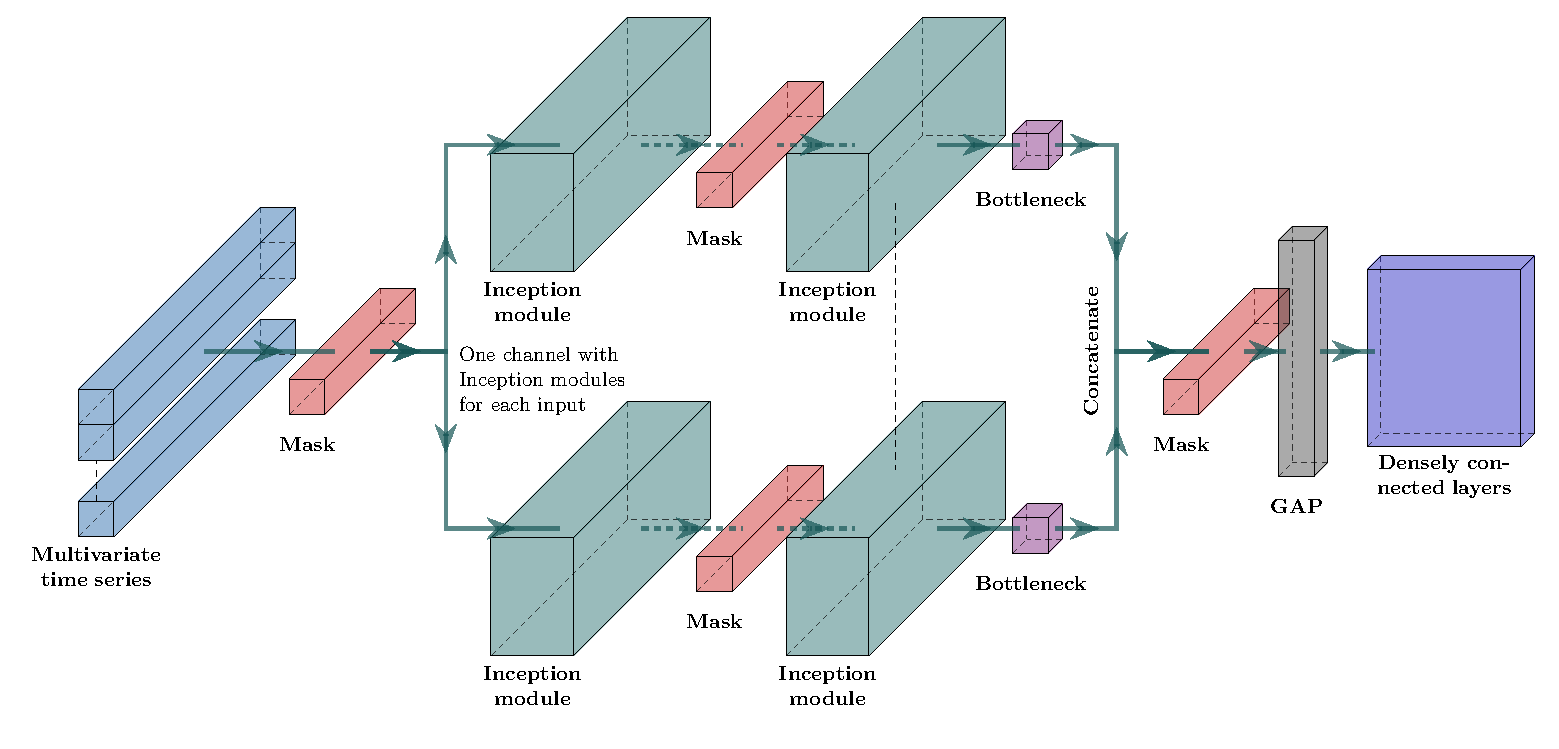
\includegraphics[width=\textwidth]{files/figs/met/x-inception-w-masks.pdf}
      {\scriptsize\textbf{Figure 6:} X-InceptionTime.}
      % \caption{}
      % \label{}
    \end{figure}

  \column{0.4\textwidth}
  \begin{block}{X-IncetionTime}
    Like InceptionTime, but input channels are kept separate.
  \end{block}
  \end{columns}

\footnotetext[14]{Fawaz et al., nceptionTime: Finding AlexNet for time series classification. 2020}
\end{frame}

\begin{frame}[fragile]{Time series classification - Ensembles}
  prata om fem modeller/poe. 2 almanna, med coral ordinal (presentera denna lite), och tre high precision models (presentera den loss function??)

  ngt mer ??

\end{frame}
\section{Results}
\begin{frame}[fragile]{Data}
  beskriv datan, typ video/reps, Antal, training/test split. Cross-val
\end{frame}
\section{Conclusions and Future work}

\begin{frame}[fragile]{Metropolis}

  The \themename theme is a Beamer theme with minimal visual noise
  inspired by the \href{https://github.com/hsrmbeamertheme/hsrmbeamertheme}{\textsc{hsrm} Beamer
  Theme} by Benjamin Weiss.

  Enable the theme by loading

  \begin{verbatim}    \documentclass{beamer}
    \usetheme{metropolis}\end{verbatim}

  Note, that you have to have Mozilla's \emph{Fira Sans} font and XeTeX
  installed to enjoy this wonderful typography.
\end{frame}
\begin{frame}[fragile]{Sections}
  Sections group slides of the same topic

  \begin{verbatim}    \section{Elements}\end{verbatim}

  for which \themename provides a nice progress indicator \ldots
\end{frame}

\section{Titleformats}

\begin{frame}{Metropolis titleformats}
	\themename supports 4 different titleformats:
	\begin{itemize}
		\item Regular
		\item \textsc{Smallcaps}
		\item \textsc{allsmallcaps}
		\item ALLCAPS
	\end{itemize}
	They can either be set at once for every title type or individually.
\end{frame}

{
    \metroset{titleformat frame=smallcaps}
\begin{frame}{Small caps}
	This frame uses the \texttt{smallcaps} titleformat.

	\begin{alertblock}{Potential Problems}
		Be aware, that not every font supports small caps. If for example you typeset your presentation with pdfTeX and the Computer Modern Sans Serif font, every text in smallcaps will be typeset with the Computer Modern Serif font instead.
	\end{alertblock}
\end{frame}
}

{
\metroset{titleformat frame=allsmallcaps}
\begin{frame}{All small caps}
	This frame uses the \texttt{allsmallcaps} titleformat.

	\begin{alertblock}{Potential problems}
		As this titleformat also uses smallcaps you face the same problems as with the \texttt{smallcaps} titleformat. Additionally this format can cause some other problems. Please refer to the documentation if you consider using it.

		As a rule of thumb: Just use it for plaintext-only titles.
	\end{alertblock}
\end{frame}
}

{
\metroset{titleformat frame=allcaps}
\begin{frame}{All caps}
	This frame uses the \texttt{allcaps} titleformat.

	\begin{alertblock}{Potential Problems}
		This titleformat is not as problematic as the \texttt{allsmallcaps} format, but basically suffers from the same deficiencies. So please have a look at the documentation if you want to use it.
	\end{alertblock}
\end{frame}
}

\section{Elements}

\begin{frame}[fragile]{Typography}
      \begin{verbatim}The theme provides sensible defaults to
\emph{emphasize} text, \alert{accent} parts
or show \textbf{bold} results.\end{verbatim}

  \begin{center}becomes\end{center}

  The theme provides sensible defaults to \emph{emphasize} text,
  \alert{accent} parts or show \textbf{bold} results.
\end{frame}

\begin{frame}{Font feature test}
  \begin{itemize}
    \item Regular
    \item \textit{Italic}
    \item \textsc{SmallCaps}
    \item \textbf{Bold}
    \item \textbf{\textit{Bold Italic}}
    \item \textbf{\textsc{Bold SmallCaps}}
    \item \texttt{Monospace}
    \item \texttt{\textit{Monospace Italic}}
    \item \texttt{\textbf{Monospace Bold}}
    \item \texttt{\textbf{\textit{Monospace Bold Italic}}}
  \end{itemize}
\end{frame}

\begin{frame}{Lists}
  \begin{columns}[T,onlytextwidth]
    \column{0.33\textwidth}
      Items
      \begin{itemize}
        \item Milk \item Eggs \item Potatos
      \end{itemize}

    \column{0.33\textwidth}
      Enumerations
      \begin{enumerate}
        \item First, \item Second and \item Last.
      \end{enumerate}

    \column{0.33\textwidth}
      Descriptions
      \begin{description}
        \item[PowerPoint] Meeh. \item[Beamer] Yeeeha.
      \end{description}
  \end{columns}
\end{frame}
\begin{frame}{Animation}
  \begin{itemize}[<+- | alert@+>]
    \item \alert<4>{This is\only<4>{ really} important}
    \item Now this
    \item And now this
  \end{itemize}
\end{frame}
\begin{frame}{Figures}
  \begin{figure}
    \newcounter{density}
    \setcounter{density}{20}
    \begin{tikzpicture}
      \def\couleur{alerted text.fg}
      \path[coordinate] (0,0)  coordinate(A)
                  ++( 90:5cm) coordinate(B)
                  ++(0:5cm) coordinate(C)
                  ++(-90:5cm) coordinate(D);
      \draw[fill=\couleur!\thedensity] (A) -- (B) -- (C) --(D) -- cycle;
      \foreach \x in {1,...,40}{%
          \pgfmathsetcounter{density}{\thedensity+20}
          \setcounter{density}{\thedensity}
          \path[coordinate] coordinate(X) at (A){};
          \path[coordinate] (A) -- (B) coordinate[pos=.10](A)
                              -- (C) coordinate[pos=.10](B)
                              -- (D) coordinate[pos=.10](C)
                              -- (X) coordinate[pos=.10](D);
          \draw[fill=\couleur!\thedensity] (A)--(B)--(C)-- (D) -- cycle;
      }
    \end{tikzpicture}
    \caption{Rotated square from
    \href{http://www.texample.net/tikz/examples/rotated-polygons/}{texample.net}.}
  \end{figure}
\end{frame}
\begin{frame}{Tables}
  \begin{table}
    \caption{Largest cities in the world (source: Wikipedia)}
    \begin{tabular}{@{} lr @{}}
      \toprule
      City & Population\\
      \midrule
      Mexico City & 20,116,842\\
      Shanghai & 19,210,000\\
      Peking & 15,796,450\\
      Istanbul & 14,160,467\\
      \bottomrule
    \end{tabular}
  \end{table}
\end{frame}
\begin{frame}{Blocks}
  Three different block environments are pre-defined and may be styled with an
  optional background color.

  \begin{columns}[T,onlytextwidth]
    \column{0.5\textwidth}
      \begin{block}{Default}
        Block content.
      \end{block}

      \begin{alertblock}{Alert}
        Block content.
      \end{alertblock}

      \begin{exampleblock}{Example}
        Block content.
      \end{exampleblock}

    \column{0.5\textwidth}

      \metroset{block=fill}

      \begin{block}{Default}
        Block content.
      \end{block}

      \begin{alertblock}{Alert}
        Block content.
      \end{alertblock}

      \begin{exampleblock}{Example}
        Block content.
      \end{exampleblock}

  \end{columns}
\end{frame}
\begin{frame}{Math}
  \begin{equation*}
    e = \lim_{n\to \infty} \left(1 + \frac{1}{n}\right)^n
  \end{equation*}
\end{frame}
\begin{frame}{Line plots}
  \begin{figure}
    \begin{tikzpicture}
      \begin{axis}[
        mlineplot,
        width=0.9\textwidth,
        height=6cm,
      ]

        \addplot {sin(deg(x))};
        \addplot+[samples=100] {sin(deg(2*x))};

      \end{axis}
    \end{tikzpicture}
  \end{figure}
\end{frame}
\begin{frame}{Bar charts}
  \begin{figure}
    \begin{tikzpicture}
      \begin{axis}[
        mbarplot,
        xlabel={Foo},
        ylabel={Bar},
        width=0.9\textwidth,
        height=6cm,
      ]

      \addplot plot coordinates {(1, 20) (2, 25) (3, 22.4) (4, 12.4)};
      \addplot plot coordinates {(1, 18) (2, 24) (3, 23.5) (4, 13.2)};
      \addplot plot coordinates {(1, 10) (2, 19) (3, 25) (4, 15.2)};

      \legend{lorem, ipsum, dolor}

      \end{axis}
    \end{tikzpicture}
  \end{figure}
\end{frame}
\begin{frame}{Quotes}
  \begin{quote}
    Veni, Vidi, Vici
  \end{quote}
\end{frame}

{%
\setbeamertemplate{frame footer}{My custom footer}
\begin{frame}[fragile]{Frame footer}
    \themename defines a custom beamer template to add a text to the footer. It can be set via
    \begin{verbatim}\setbeamertemplate{frame footer}{My custom footer}\end{verbatim}
\end{frame}
}

% \begin{frame}{References}
%   Some references to showcase [allowframebreaks] \cite{knuth92,ConcreteMath,Simpson,Er01,greenwade93}
% \end{frame}

\section{Conclusion}

\begin{frame}{Summary}

  Get the source of this theme and the demo presentation from

  \begin{center}\url{github.com/matze/mtheme}\end{center}

  The theme \emph{itself} is licensed under a
  \href{http://creativecommons.org/licenses/by-sa/4.0/}{Creative Commons
  Attribution-ShareAlike 4.0 International License}.

  \begin{center}\ccbysa\end{center}

\end{frame}

\begin{frame}[standout]
  Questions?
\end{frame}

\appendix

\begin{frame}[fragile]{Backup slides}
  Sometimes, it is useful to add slides at the end of your presentation to
  refer to during audience questions.

  The best way to do this is to include the \verb|appendixnumberbeamer|
  package in your preamble and call \verb|\appendix| before your backup slides.

  \themename will automatically turn off slide numbering and progress bars for
  slides in the appendix.
\end{frame}

\begin{frame}[allowframebreaks]{References}

  % \bibliography{demo}
  \bibliographystyle{abbrv}
  \printbibliography

\end{frame}

\end{document}
